\documentclass[border=4pt]{standalone}
\usepackage{tikz}
\usetikzlibrary{decorations.pathreplacing}
\begin{document}
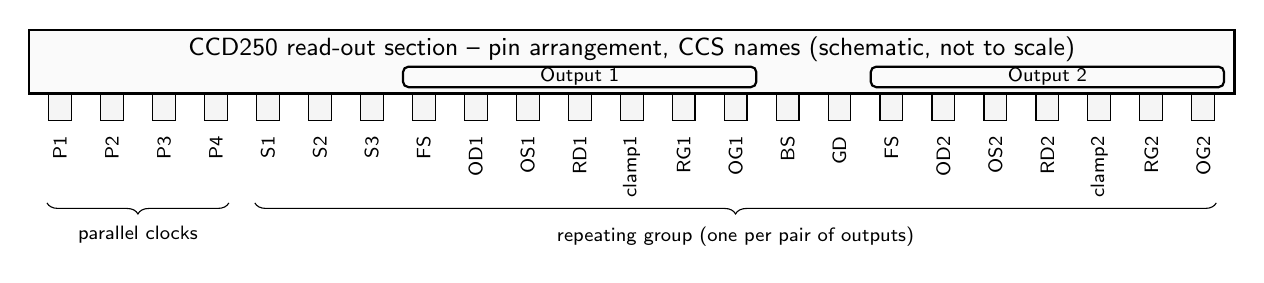
\begin{tikzpicture}[x=0.66cm,y=1cm,font=\sffamily]
  \foreach \p [count=\i from 0] in {P1,P2,P3,P4,S1,S2,S3,FS,OD1,OS1,RD1,clamp1,RG1,OG1,BS,GD,FS,OD2,OS2,RD2,clamp2,RG2,OG2} {
    \draw[fill=black!4] (\i-0.22,0) rectangle (\i+0.22,0.34);
    \node[anchor=east,rotate=90,font=\sffamily\scriptsize] at (\i,-0.08) {\p};
  }
  \draw[thick,fill=black!2] (-0.6,0.34) rectangle (22.6,1.15);
  \node[font=\sffamily\small] at (11,0.9) {CCD250 read-out section -- pin arrangement, CCS names (schematic, not to scale)};
  \draw[thick,rounded corners=2pt] (6.6,0.42) rectangle (13.4,0.68);
  \node[font=\sffamily\scriptsize] at (10,0.55) {Output 1};
  \draw[thick,rounded corners=2pt] (15.6,0.42) rectangle (22.4,0.68);
  \node[font=\sffamily\scriptsize] at (19,0.55) {Output 2};
  \draw[decorate,decoration={brace,amplitude=4pt,mirror}]
       (-0.25,-1.05) -- (3.25,-1.05)
       node[midway,below=5pt,font=\sffamily\scriptsize] {parallel clocks};
  \draw[decorate,decoration={brace,amplitude=4pt,mirror}]
       (3.75,-1.05) -- (22.25,-1.05)
       node[midway,below=5pt,font=\sffamily\scriptsize]
       {repeating group (one per pair of outputs)};
\end{tikzpicture}
\end{document}
